
%% bare_conf.tex
%% V1.4b
%% 2015/08/26
%% by Michael Shell
%% See:
%% http://www.michaelshell.org/
%% for current contact information.
%%
%% This is a skeleton file demonstrating the use of IEEEtran.cls
%% (requires IEEEtran.cls version 1.8b or later) with an IEEE
%% conference paper.
%%
%% Support sites:
%% http://www.michaelshell.org/tex/ieeetran/
%% http://www.ctan.org/pkg/ieeetran
%% and
%% http://www.ieee.org/

%%*************************************************************************
%% Legal Notice:
%% This code is offered as-is without any warranty either expressed or
%% implied; without even the implied warranty of MERCHANTABILITY or
%% FITNESS FOR A PARTICULAR PURPOSE!
%% User assumes all risk.
%% In no event shall the IEEE or any contributor to this code be liable for
%% any damages or losses, including, but not limited to, incidental,
%% consequential, or any other damages, resulting from the use or misuse
%% of any information contained here.
%%
%% All comments are the opinions of their respective authors and are not
%% necessarily endorsed by the IEEE.
%%
%% This work is distributed under the LaTeX Project Public License (LPPL)
%% ( http://www.latex-project.org/ ) version 1.3, and may be freely used,
%% distributed and modified. A copy of the LPPL, version 1.3, is included
%% in the base LaTeX documentation of all distributions of LaTeX released
%% 2003/12/01 or later.
%% Retain all contribution notices and credits.
%% ** Modified files should be clearly indicated as such, including  **
%% ** renaming them and changing author support contact information. **
%%*************************************************************************


% *** Authors should verify (and, if needed, correct) their LaTeX system  ***
% *** with the testflow diagnostic prior to trusting their LaTeX platform ***
% *** with production work. The IEEE's font choices and paper sizes can   ***
% *** trigger bugs that do not appear when using other class files.       ***                          ***
% The testflow support page is at:
% http://www.michaelshell.org/tex/testflow/



\documentclass[conference]{IEEEtran}
% Some Computer Society conferences also require the compsoc mode option,
% but others use the standard conference format.
%
% If IEEEtran.cls has not been installed into the LaTeX system files,
% manually specify the path to it like:
% \documentclass[conference]{../sty/IEEEtran}





% Some very useful LaTeX packages include:
% (uncomment the ones you want to load)


% *** MISC UTILITY PACKAGES ***
%
%\usepackage{ifpdf}
% Heiko Oberdiek's ifpdf.sty is very useful if you need conditional
% compilation based on whether the output is pdf or dvi.
% usage:
% \ifpdf
%   % pdf code
% \else
%   % dvi code
% \fi
% The latest version of ifpdf.sty can be obtained from:
% http://www.ctan.org/pkg/ifpdf
% Also, note that IEEEtran.cls V1.7 and later provides a builtin
% \ifCLASSINFOpdf conditional that works the same way.
% When switching from latex to pdflatex and vice-versa, the compiler may
% have to be run twice to clear warning/error messages.






% *** CITATION PACKAGES ***
%
\usepackage{cite}
% cite.sty was written by Donald Arseneau
% V1.6 and later of IEEEtran pre-defines the format of the cite.sty package
% \cite{} output to follow that of the IEEE. Loading the cite package will
% result in citation numbers being automatically sorted and properly
% "compressed/ranged". e.g., [1], [9], [2], [7], [5], [6] without using
% cite.sty will become [1], [2], [5]--[7], [9] using cite.sty. cite.sty's
% \cite will automatically add leading space, if needed. Use cite.sty's
% noadjust option (cite.sty V3.8 and later) if you want to turn this off
% such as if a citation ever needs to be enclosed in parenthesis.
% cite.sty is already installed on most LaTeX systems. Be sure and use
% version 5.0 (2009-03-20) and later if using hyperref.sty.
% The latest version can be obtained at:
% http://www.ctan.org/pkg/cite
% The documentation is contained in the cite.sty file itself.






% *** GRAPHICS RELATED PACKAGES ***
%
\ifCLASSINFOpdf
  \usepackage[pdftex]{graphicx}
  % declare the path(s) where your graphic files are
  % \graphicspath{{../pdf/}{../jpeg/}}
  % and their extensions so you won't have to specify these with
  % every instance of \includegraphics
  % \DeclareGraphicsExtensions{.pdf,.jpeg,.png}
\else
  % or other class option (dvipsone, dvipdf, if not using dvips). graphicx
  % will default to the driver specified in the system graphics.cfg if no
  % driver is specified.
  % \usepackage[dvips]{graphicx}
  % declare the path(s) where your graphic files are
  % \graphicspath{{../eps/}}
  % and their extensions so you won't have to specify these with
  % every instance of \includegraphics
  % \DeclareGraphicsExtensions{.eps}
\fi
% graphicx was written by David Carlisle and Sebastian Rahtz. It is
% required if you want graphics, photos, etc. graphicx.sty is already
% installed on most LaTeX systems. The latest version and documentation
% can be obtained at:
% http://www.ctan.org/pkg/graphicx
% Another good source of documentation is "Using Imported Graphics in
% LaTeX2e" by Keith Reckdahl which can be found at:
% http://www.ctan.org/pkg/epslatex
%
% latex, and pdflatex in dvi mode, support graphics in encapsulated
% postscript (.eps) format. pdflatex in pdf mode supports graphics
% in .pdf, .jpeg, .png and .mps (metapost) formats. Users should ensure
% that all non-photo figures use a vector format (.eps, .pdf, .mps) and
% not a bitmapped formats (.jpeg, .png). The IEEE frowns on bitmapped formats
% which can result in "jaggedy"/blurry rendering of lines and letters as
% well as large increases in file sizes.
%
% You can find documentation about the pdfTeX application at:
% http://www.tug.org/applications/pdftex





% *** MATH PACKAGES ***
%
%\usepackage{amsmath}
% A popular package from the American Mathematical Society that provides
% many useful and powerful commands for dealing with mathematics.
%
% Note that the amsmath package sets \interdisplaylinepenalty to 10000
% thus preventing page breaks from occurring within multiline equations. Use:
%\interdisplaylinepenalty=2500
% after loading amsmath to restore such page breaks as IEEEtran.cls normally
% does. amsmath.sty is already installed on most LaTeX systems. The latest
% version and documentation can be obtained at:
% http://www.ctan.org/pkg/amsmath

\usepackage{bm}
\usepackage{amsthm}
\usepackage{amsmath}
\usepackage{amsfonts}
\newcommand{\Z}{\mathbb Z}
\newcommand{\N}{\mathbb N}
\newcommand{\B}{\mathrm{B}}

%\newtheorem{Def}{Definition}
%\newtheorem{Lem}{Lemma}
%\newtheorem{Cor}[Lem]{Corollary}
%\newtheorem*{Th}{Theorem}
\newtheorem*{Prop}{Proposition}

% *** SPECIALIZED LIST PACKAGES ***
%
%\usepackage{algorithmic}
% algorithmic.sty was written by Peter Williams and Rogerio Brito.
% This package provides an algorithmic environment fo describing algorithms.
% You can use the algorithmic environment in-text or within a figure
% environment to provide for a floating algorithm. Do NOT use the algorithm
% floating environment provided by algorithm.sty (by the same authors) or
% algorithm2e.sty (by Christophe Fiorio) as the IEEE does not use dedicated
% algorithm float types and packages that provide these will not provide
% correct IEEE style captions. The latest version and documentation of
% algorithmic.sty can be obtained at:
% http://www.ctan.org/pkg/algorithms
% Also of interest may be the (relatively newer and more customizable)
% algorithmicx.sty package by Szasz Janos:
% http://www.ctan.org/pkg/algorithmicx




% *** ALIGNMENT PACKAGES ***
%
%\usepackage{array}
% Frank Mittelbach's and David Carlisle's array.sty patches and improves
% the standard LaTeX2e array and tabular environments to provide better
% appearance and additional user controls. As the default LaTeX2e table
% generation code is lacking to the point of almost being broken with
% respect to the quality of the end results, all users are strongly
% advised to use an enhanced (at the very least that provided by array.sty)
% set of table tools. array.sty is already installed on most systems. The
% latest version and documentation can be obtained at:
% http://www.ctan.org/pkg/array


% IEEEtran contains the IEEEeqnarray family of commands that can be used to
% generate multiline equations as well as matrices, tables, etc., of high
% quality.




% *** SUBFIGURE PACKAGES ***
%\ifCLASSOPTIONcompsoc
%  \usepackage[caption=false,font=normalsize,labelfont=sf,textfont=sf]{subfig}
%\else
%  \usepackage[caption=false,font=footnotesize]{subfig}
%\fi
% subfig.sty, written by Steven Douglas Cochran, is the modern replacement
% for subfigure.sty, the latter of which is no longer maintained and is
% incompatible with some LaTeX packages including fixltx2e. However,
% subfig.sty requires and automatically loads Axel Sommerfeldt's caption.sty
% which will override IEEEtran.cls' handling of captions and this will result
% in non-IEEE style figure/table captions. To prevent this problem, be sure
% and invoke subfig.sty's "caption=false" package option (available since
% subfig.sty version 1.3, 2005/06/28) as this is will preserve IEEEtran.cls
% handling of captions.
% Note that the Computer Society format requires a larger sans serif font
% than the serif footnote size font used in traditional IEEE formatting
% and thus the need to invoke different subfig.sty package options depending
% on whether compsoc mode has been enabled.
%
% The latest version and documentation of subfig.sty can be obtained at:
% http://www.ctan.org/pkg/subfig




% *** FLOAT PACKAGES ***
%
%\usepackage{fixltx2e}
% fixltx2e, the successor to the earlier fix2col.sty, was written by
% Frank Mittelbach and David Carlisle. This package corrects a few problems
% in the LaTeX2e kernel, the most notable of which is that in current
% LaTeX2e releases, the ordering of single and double column floats is not
% guaranteed to be preserved. Thus, an unpatched LaTeX2e can allow a
% single column figure to be placed prior to an earlier double column
% figure.
% Be aware that LaTeX2e kernels dated 2015 and later have fixltx2e.sty's
% corrections already built into the system in which case a warning will
% be issued if an attempt is made to load fixltx2e.sty as it is no longer
% needed.
% The latest version and documentation can be found at:
% http://www.ctan.org/pkg/fixltx2e


%\usepackage{stfloats}
% stfloats.sty was written by Sigitas Tolusis. This package gives LaTeX2e
% the ability to do double column floats at the bottom of the page as well
% as the top. (e.g., "\begin{figure*}[!b]" is not normally possible in
% LaTeX2e). It also provides a command:
%\fnbelowfloat
% to enable the placement of footnotes below bottom floats (the standard
% LaTeX2e kernel puts them above bottom floats). This is an invasive package
% which rewrites many portions of the LaTeX2e float routines. It may not work
% with other packages that modify the LaTeX2e float routines. The latest
% version and documentation can be obtained at:
% http://www.ctan.org/pkg/stfloats
% Do not use the stfloats baselinefloat ability as the IEEE does not allow
% \baselineskip to stretch. Authors submitting work to the IEEE should note
% that the IEEE rarely uses double column equations and that authors should try
% to avoid such use. Do not be tempted to use the cuted.sty or midfloat.sty
% packages (also by Sigitas Tolusis) as the IEEE does not format its papers in
% such ways.
% Do not attempt to use stfloats with fixltx2e as they are incompatible.
% Instead, use Morten Hogholm'a dblfloatfix which combines the features
% of both fixltx2e and stfloats:
%
% \usepackage{dblfloatfix}
% The latest version can be found at:
% http://www.ctan.org/pkg/dblfloatfix




% *** PDF, URL AND HYPERLINK PACKAGES ***
%
\usepackage{url}
% url.sty was written by Donald Arseneau. It provides better support for
% handling and breaking URLs. url.sty is already installed on most LaTeX
% systems. The latest version and documentation can be obtained at:
% http://www.ctan.org/pkg/url
% Basically, \url{my_url_here}.


\usepackage{svg}

% *** Do not adjust lengths that control margins, column widths, etc. ***
% *** Do not use packages that alter fonts (such as pslatex).         ***
% There should be no need to do such things with IEEEtran.cls V1.6 and later.
% (Unless specifically asked to do so by the journal or conference you plan
% to submit to, of course. )


% correct bad hyphenation here
\hyphenation{op-tical net-works semi-conduc-tor}


\begin{document}
%
% paper title
% Titles are generally capitalized except for words such as a, an, and, as,
% at, but, by, for, in, nor, of, on, or, the, to and up, which are usually
% not capitalized unless they are the first or last word of the title.
% Linebreaks \\ can be used within to get better formatting as desired.
% Do not put math or special symbols in the title.
\title{Constructing Large-scale Low-latency Network from Small Optimal Networks}


% author names and affiliations
% use a multiple column layout for up to three different
% affiliations
\author{\IEEEauthorblockN{Ryosuke Mizuno}
\IEEEauthorblockA{Department of Physics\\
 Kyoto University, Kyoto, Japan\\
Email: mizuno@tap.scphys.kyoto-u.ac.jp}
\and
\IEEEauthorblockN{Yawara Ishida}
\IEEEauthorblockA{Research Institute for Mathematical Science\\
Kyoto University, Kyoto, Japan\\
Email: yawara@kurims.kyoto-u.ac.jp}
}

% conference papers do not typically use \thanks and this command
% is locked out in conference mode. If really needed, such as for
% the acknowledgment of grants, issue a \IEEEoverridecommandlockouts
% after \documentclass

% for over three affiliations, or if they all won't fit within the width
% of the page, use this alternative format:
%
%\author{\IEEEauthorblockN{Michael Shell\IEEEauthorrefmark{1},
%Homer Simpson\IEEEauthorrefmark{2},
%James Kirk\IEEEauthorrefmark{3},
%Montgomery Scott\IEEEauthorrefmark{3} and
%Eldon Tyrell\IEEEauthorrefmark{4}}
%\IEEEauthorblockA{\IEEEauthorrefmark{1}School of Electrical and Computer Engineering\\
%Georgia Institute of Technology,
%Atlanta, Georgia 30332--0250\\ Email: see http://www.michaelshell.org/contact.html}
%\IEEEauthorblockA{\IEEEauthorrefmark{2}Twentieth Century Fox, Springfield, USA\\
%Email: homer@thesimpsons.com}
%\IEEEauthorblockA{\IEEEauthorrefmark{3}Starfleet Academy, San Francisco, California 96678-2391\\
%Telephone: (800) 555--1212, Fax: (888) 555--1212}
%\IEEEauthorblockA{\IEEEauthorrefmark{4}Tyrell Inc., 123 Replicant Street, Los Angeles, California 90210--4321}}




% use for special paper notices
%\IEEEspecialpapernotice{(Invited Paper)}




% make the title area
\maketitle

% As a general rule, do not put math, special symbols or citations
% in the abstract
\begin{abstract}
The construction of large-scale, low-latency networks becomes difficult as the number of nodes increases.
In general, the way to construct a theoretically optimal solution is unknown.
However, it is known that some methods can construct suboptimal networks with low-latency.
One such method is to construct large-scale networks from optimal or suboptimal small networks, using the product of graphs.
There are two major advantages to this method.
One is that we can reuse small, already known networks to construct large-scale networks.
The other is that the networks obtained by this method have graph-theoretical symmetry, 
which reduces the overhead of communication between nodes.
A network can be viewed as a ``graph'', which is a mathematical term from combinatorics.
The design of low-latency networks can be treated as a mathematical problem 
of finding small diameter graphs with a given number of nodes ( called ``order'' )
and a given number of connections between each node ( called ``degree'' ).
In this paper, we overview how to construct large graphs from optimal or suboptimal small graphs by using graph-theoretical products.
We focus on the case of diameter 2 in particular.
As an example, we introduce a graph of order 256, degree 22 and diameter 2,
which granted us the Deepest Improvement Award at the ``Graph Golf'' competition.
Moreover, the average shortest path length of the graph is the smallest in graphs of order 256 and degree 22. 
\end{abstract}

\begin{IEEEkeywords}
low-latency network, graph theory, the degree-diameter problem, the order-degree problem, Brown's construction, star product.
\end{IEEEkeywords}

% no keywords




% For peer review papers, you can put extra information on the cover
% page as needed:
% \ifCLASSOPTIONpeerreview
% \begin{center} \bfseries EDICS Category: 3-BBND \end{center}
% \fi
%
% For peerreview papers, this IEEEtran command inserts a page break and
% creates the second title. It will be ignored for other modes.
\IEEEpeerreviewmaketitle



\section{Introduction}
% no \IEEEPARstart
In mathematics, graph theory is the study of graphs, which are mathematical objects
obtained by abstraction of networks.
A {\it graph} $G$ is a network which consists of a set of {\it vertices} $V$ and of {\it edges} $E$.
Nodes and connections between nodes are translated to vertices and edges respectively.
Two distinct vertices $u$ and $v$ of $G$ are connected to each other
if and only if $(u,v) \in E$. 
In this case, we say that $u$ and $v$ are {\it adjacent} and use the notation $u \sim v$.
For example, let $V$ be a set of $(i,j)$ such that $i = 0,1$ and $j=0,1, \ldots ,4$, and let $E$ be a set of $((i,j),(k,l))$
such that if $i=k$ then $j=l \pm 1 \bmod 5$ or if $i \neq k$ then $j = 2l \bmod 5$.
The graph of the given $V$ and $E$ is called {\it Petersen graph} as shown in Figure~\ref{fig:Petersen}.
\begin{figure}[]
\centering
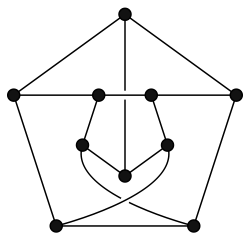
\includegraphics[width=3cm]{petersen_gray.png}
\caption{ Petersen graph.}
\label{fig:Petersen}
\end{figure}
We can study networks by modeling them as graphs and formulate various problems in terms of graph theory.
For example, the traveling salesman problem, the four color theorem, the max-flow min-cut theorem
and the shortest path problem are well known formulations of problems of networks.
Knowledge gained by the formulation of graph theory is expected to be useful for the study of networks.

The {\it order} $N=|G|=|V|$ and the {\it maximum degree} of vertices $\Delta$ are basic feature values of
graphs, where the degree of a vertex is the number of adjacent vertices to it.
The {\it distance} $d(u,v)$ between $u$ and $v$ in $V$  is the length of the shortest path between them.
The {\it diameter} $D$ of the graph $G$ is the maximum distance of all pairs of vertices;
\[ D = \max_{u,  v \in V} d(u,v). \]
The diameter of Petersen graph is $2$.
Let us turn to some other famous examples of graphs.
Let $V$ be vertices of the $n$-dimensional hypercube over a field such that each component is $1$ or $0$,
and the vertices ${\bm x}$ and ${\bm y}$ in $V$ are adjacent if and only if $1$ or $-1$ appears just once in the components of ${\bm x}-{\bm y}$, and other components of it are $0$.
This graph is called an {\it $n$-dimensional hypercube graph},
which is of $N=2^n, \Delta=n, D=n$.
Let $V$ be ${(\Z/m\Z)}^n$ such that $m > 2$, and two vertices ${\bm x}$ and ${\bm y}$ in $V$ are adjacent
if and only if $1$ or $m-1$ appears just once in the components of ${\bm x}-{\bm y}$, and other components of it are $0$.
This graph is called an {\it $n$-dimensional torus grid graph},
which is of $N=m^n, \Delta=2n, D=n [m/2]$ where this bracket is gauss's symbol.
These two examples are graphs obtained by abstracting known topological structures.
On the other hand, we can also construct graphs directly by using algebraic methods.
Let $L$ be a set of distinct $t$ labels and let the vertices $V$ be $L^n$.
The vertices $(a_1, a_2, \ldots, a_n)$ and $(b_1, b_2, \ldots, b_n)$ in $V$ are adjacent if and only if $a_i = b_{i+1}$ or $a_{i+1} = b_i$ for $i=1,2, \ldots k-1$.
This graph is known as undirected {\it de Brujin graph} of type $(t,n)$
of $N=t^n, \Delta=2t, D=n$~\cite{bruijn1946combinatorial,good1946normal}.

The order, the maximum degree, and the diameter are important indices for measuring
the efficiency of connections between vertices of a graph.
If a graph of given diameter and maximum degree has more vertices, we consider it as a more efficient network.
This claim can be rephrased into two other forms.
One is that a graph of given order and maximum degree is more dense if its diameter is smaller.
The other is that if the maximum degree of a graph of given order and diameter is smaller,
the distribution of the edges is more efficient.
These claims correspond to three optimization problems; {\it the degree-diameter problem},
{\it the order-degree problem} and {\it the order-diameter problem}.
The degree-diameter problem is to find the largest possible number of vertices in a graph of given degree and diameter~\cite{MilSir2005}.
Of the above three, this is the most attractive to mathematicians.
A table of a lower bound of the largest possible number of vertices with given degree and diameter is available online at the Combinatorics Wiki website \cite{combinatoricswiki}.
The order-degree problem is to find graphs with the smallest diameter in graphs of given order and degree.
This problem can be applied for designing of law-latency networks, but a table similar to the degree-diameter problem has not been constructed as of yet. 
Only a very small table is available online at the Graph Golf website \cite{graphgolf}.
The order-degree problem is to find graphs with the smallest maximum degree in a graph of given order and diameter.
Unfortunately, this problem has been somewhat overlooked compared to the others.
These three problems are strongly interrelated.
Therefore we can use the best-studied degree-diameter problem in order to study the others.
In what follows, we review the degree-diameter problem and two methods for constructing graphs of diameter $2$ for the order-degree problem.
One is {\it Brown's construction}, which was originally introduced by W.G. Brown ~\cite{brown1966graphs}
and later generalized by the co-author\cite{gbc} of this paper.
The other is graph-theoretical product known as {\it star product}\cite{bermond1982large,MilSir2005}.
This allows us to introduce the graph of order $256$, degree $22$, and diameter $2$.
Moreover, the average shortest path length of the graph is the smallest in graphs of order $256$ and degree $22$,
where the average shortest path length $ASPL$ is defined as follows;
\[ ASPL = \frac{\sum_{u, v \in V} d(u, v)}{|V| (|V| -1)} \]

\section{The degree-diameter problem}
As mentioned above, the degree-diameter problem is to find
the largest possible number  $n_{\Delta,D}$ of vertices in a graph of given degree $\Delta$ and diameter $D$~\cite{MilSir2005}.
If $G$ is a graph with degree $\Delta$ and diameter $D$, then we get
\[ |G| \leq n_{\Delta,D} \leq 1 + \Delta \sum_{k=0}^{D-1} (\Delta - 1)^k\]
where $|G|$ is the number of vertices of $G$.
The right hand side of the above inequality is called {\it Moore bound}.
The graph whose order equals Moore bound is called {\it Moore graph}.
In the case of $D=2$, Moore graph can exists when $\Delta=2, 3, 7, 57$~\cite{hoffman1960moore}.
In fact, if $\Delta=2, 3, 7$, then Moore graphs are a pentagon, Petersen graph, Hoffman-Singleton graph respectively.
It is not known whether Moore graph exists if $\Delta=57$.
In the case of $D \geq 3$, Moore graph is a cycle graph of length $2D+1$~\cite{damerell1973moore}.
Some general lower bounds of $n_{\Delta, D}$ are known( see ~\cite{MilSir2005} ).
For example, if $\Delta$ is an even number, the undirected de Brujin graph gives a lower bound of $n_{\Delta, D}$;
\[ n_{\Delta, D} \geq {\left( \frac{\Delta}{2} \right)}^D \]

However, exact lower bounds of $n_{\Delta, D}$ are only known for small $\Delta, D$.
Thus, the order-diameter problem for almost all pairs of $\Delta, D$ is unsolved.
Let us consider the case of $\Delta=8, D=8$, where Moore bound is $7686401$.
The $8$-dimensional hypercube graph, the $4$-dimensional torus grid graph over $\Z/5\Z$,
and the undirect de Brujin graph of type $(4,8)$ are examples of $\Delta=8,D=8$.
The order of the $8$-dimensional hypercube graph is $2^8=256$.
The order of the $4$-dimensional torus grid graph over $\Z/5\Z$ is $5^4=625$, 
which is more efficient than $8$-dimensional hypercube.
The order of undirect de Brujin graph of type $(4,8)$ is $4^8=65536$,
which is more efficient than the above two graphs.
The order of the already known suboptimal graph of $\Delta=8, D=8$ is $734820$~\cite{Loz08newrecord}.
The graph is discovered by using a computer.
However it seems to be too small because the percentage of the Moore bound for $\Delta=8, D=8$ is $9.56$\%.
As another example, let us consider the case of $\Delta=20, D=2$.
The order the undirected de Brujin graph of type $(10, 2)$ of $\Delta=20, D=2$ is $10^2=100$.
The order of the already known suboptimal graph  of $\Delta=20, D=2$ is $381$,
where the percentage of the Moore bound for $\Delta=20, D=2$ is $95$\%.
It is obtained by Brown's Construction, which we will discuss in more detail later on.
As mentioned above, the hypercube graph, the torus grid graph, and the de Brujin graph are very simple and easy to construct,
but these graphs are not close to suboptimal.
Thus, when we want more dense or more efficient graphs, these simple graphs are not suitable.
In order to construct more dense or more efficient graphs, there are roughly two ways;
either by a deterministic mathematical construction, or by searching suboptimal graphs using computers.
Furthermore, a deterministic mathematical construction can be divided into two ways.
One way is to construct graphs with more vertices from scratch.
The other is to construct graphs from small, already known suboptimal graphs.

\subsection{The case of diameter $2$}
For the case of diameter $2$, Brown's construction~\cite{brown1966graphs,MilSir2005} gives suboptimal graphs.
This construction gives a graph for each $q$ which is a power of a prime.
Let $F_q$ be a finite field.
Brown's construction gives the graph $\B(F_q)$ where the vertices are lines in $F_q^3$ and two lines are adjacent if and only if they are orthogonal.
It follows that;
\[ |\B(F_q)| = q^2+q+1, \quad \Delta(\B(F_q)) = q+1, \quad D(\B(F_q))=2.\]
The degree of each vertex of $\B(F_q)$ is $q+1$ or $q$.
The reason of $D(\B(F_q))=2$ is that
for all two vectors ${\bm x}$ and ${\bm y}$ there exists a vector ${\bm z}$ orthogonal to ${\bm x}$ and ${\bm y}$ even in finite vector spaces.
Therefore, for ${\Delta}$, if a power of a prime $q$ exists such that $\Delta=q+1$, we get
\[ n_{\Delta, D} \geq \Delta^2 - \Delta + 1. \]
Among $q^2+q+1$ vertices, $q+1$ vertices are of degree $q$ and $q^2$ vertices are of degree $q+1$.
If $q$ is a power of $2$, there exists the graph of $N=q^2+q+2, \Delta=q+1,D=2$~\cite{journals/networks/ErdosFH80}.
Therefore, if $\Delta$ is a power of 2, we have
\[ n_{\Delta, D} \geq \Delta^2 - \Delta + 2. \]
For the remainder $\Delta$, we get suboptimal graphs by duplicating the vertex of the graphs obtained by Brown's construction~\cite{MilSir2005}.
For any $\epsilon >0$ there exists a constant $c_\epsilon$ such that, for any $\Delta$ the following holds;
\[ n_{\Delta, D} \geq \Delta^2 - c_\epsilon \Delta^{19/12+\epsilon}. \]
For the case of diameter $2$ with large maximum degree, the graphs obtained by Brown's construction
are the best suboptimal graphs among already known graphs.

Let us turn to another graph-theoretical technique known as star product, which was introduced by Bermond, Delorme and Farhi\cite{bermond1982large,MilSir2005}.
Let $G_1, G_2$ be graphs.
We fix an arbitrary orientation of all edges of $G_1$ and let $\vec{E}$ be the corresponding set of the fixed arrows of $G_1$.
For each arrow $(u,v) \in \vec{E}$, let $\phi(u,v)$ be a bijection on the set $V(G_2)$.
The vertex set of the star product $G_1 *_\phi G_2$ is thus $V(G_1) \times V(G_2)$,
and the vertex $(u, v)$ is adjacent to $(w, x)$ if and only if either $u = w$ and $(v,x)$ is an edge of $G_2$, or
$(u, w)$ is in $\vec{E}$ and $x=\phi(u,w)(v)$.
Using this product, we can construct some efficient graphs.
For example, we can construct the graph that gives the exact lower bound of order for $\Delta=6, D=2$.
The exact lower bound for $\Delta=6, D=2$ is 32, namely $n_{6,2} = 32$.
Let the graph $G_8$ of order $8$ be as follows;
\[ V=\{(0,0),(0,1),(1,0),(1,1),(1,2),(2,0),(2,1),(2,2)\} \]
and $(i,j), (k,l)$ in $V$ be adjacent if and only if
$(i,k)$ in $\{ (0,1),(1,0),(2,2)\}$, or if $(i,k)=(1,2),(2,1)$ then $j=l$.
$G_8$ is of order $8$, degree $8$, and diameter $2$ as shown in Figure~\ref{fig:g8}.
\begin{figure}[]
\centering
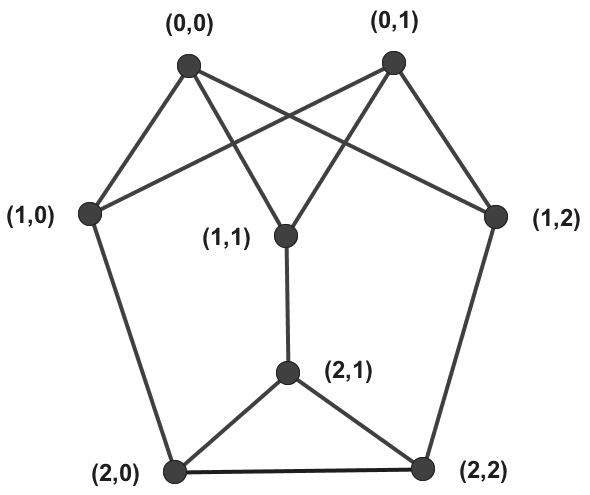
\includegraphics[width=5cm]{g8.png}
\caption{ The $G_8$ Construction.}
\label{fig:g8}
\end{figure}
Let $K_n$ be a $n$-complete graph, where each vertex is connected to all other vertices.
The vertices of $K_n$ is labeled by natural numbers, namely $V(K_n)=\{0,1,\ldots, n-1\}$.
Let $\vec{E}$ be $\{(k_1,k_2)| k_1 < k_2\}$ and $\phi$ be defined as follows;
\[
  \phi(k_1,k_2)((i,j)) =
    \begin{cases}
      (0,1-j) & (i=0) \\
      (2,j+1 \bmod 3) & (i=1) \\
      (1,j-1 \bmod 3) & (i=2).
    \end{cases}
\]
Then we get the star product $K_n *_\phi G_8$ with $\phi$, which is of order $8n$, degree $n+2$ such that if $n \geq 3$, the diameter is $2$.
When $n=4$, the $K_4 *_\phi G_8$ is the optimal graph of order $32$ for the degree-diameter problem of $\Delta=6, D=2$.

\section{The order-degree problem}
The order-degree problem is to find the graph with the smallest diameter in graphs of given order and degree.
As mentioned above, the order-degree problem is correlated strongly with the degree-diameter problem.
In fact, for given degree $\Delta$ and diameter $D$, the optimal graph $G$ for the degree-diameter problem is also
optimal for the order-degree problem of order $|G|$ and degree $\Delta$.
If $G$ is not optimal for the order-degree problem, then there exists the graph $G'$ of order $|G|$, degree $\Delta$ and diameter $D' < D$.
Thus, we get $G''$ of order $|G|+1$, degree $\Delta$ and $D'+1 \leq D$ by inserting one vertex into an arbitrary edge of $G'$.
This contradicts the assumption that $G$ is the largest graph of given degree $\Delta$ and diameter $D$.
Therefore, the already known suboptimal graphs  for degree-diameter problem seem to be suboptimal for order-degree problem.
However, the order of optimal or suboptimal graphs of the degree-diameter problem does not cover an arbitrary order.
For example, the facts of $n_{6,2}=32$ and $n_{7,2}=50$ implies nothing more than
 that if $33 \leq |G| \leq 49$ and $D=2$, then $\Delta \geq 7$, or if $33 \leq |G| \leq 49$ and $\Delta=6$, then $D \geq 3$.
Namely, the graphs obtained from the degree-diameter problem cover a very limited number of pairs of order and degree for the order-degree problem.
Thus, we have to construct graphs for missing pairs of given order and degree.
As well as the degree-diameter problem, there are roughly two deterministic ways to construct graphs;
to construct graphs from scratch or from already known small graphs.
We introduce two ways corresponding to them; generalized Brown's construction and multiple star product,
which are the generalization of Brown's construction and star product respectively.
Using multiple star product, we construct the graph of order $256$, degree $22$, and diameter $2$.

\subsection{Generalized Brown's Construction}
We give a generalization of Brown's construction~\cite{gbc} by replacing a finite field $F_q$ with a finite commutative ring $R$ with unity, in particular $\Z/n\Z$.
The vertices $V(\B(R))$ is defined as follows;
\[( R^3 \setminus \{\bm v | \exists r \in R, r \cdot {\bm v} = {\bm 0} \} ) / \sim\]
where $\bm v \sim \bm w$ if and only if there exists $k \in R^*$ such that $k \cdot {\bm v} = {\bm w}$.
The two vertices $[\bm v]$ and $[\bm w]$ are adjacent if and only if ${\bm v} \cdot {\bm w} = 0$.
It is clear that, if $R$ is finite, then so is $\B(R)$.
Moreover if $R$ is a quotient of any Euclidean domain, then the diameter of $\B(R)$ is $2$.
When $R=\Z/n\Z$, there exist prime numbers $p_i$ and natural numbers $k_i > 0$ such that $n=\prod_{i} {p_i}^{k_i}$,
and it follows that;
\[ |\B(\Z/n\Z)| = \prod_i \left( {p_i}^{2k_i}+{p_i}^{2k_i-1}+{p_i}^{2k_i-2} \right)\]
\[ \Delta(\B(\Z/n\Z)) = \prod_i \left( {p_i}^{k_i} + {p_i}^{k_i-1} \right). \]
\[ D(\B(\Z/n\Z)) = 2\]
Therefore, for given order $N$ and degree $\Delta$, if there exists a natural number $n \geq 2$ and $\delta \geq 0$
such that $N=|\B(\Z/n\Z)|+\delta$ and $\Delta \geq \Delta(\B(\Z/n\Z))+\delta$, 
then we have the graph of order $N$, degree $\Delta$ and diameter $2$
by $\delta$ times duplicating vertices of $\B(\Z/n\Z)$ and adding some edges.
We omit the proof of the above discussion because the details will appear in our next paper\cite{nextpaper}.

\subsection{Multiple Star Product}
Let us construct the graph of order $256$, degree $22$, and diameter $2$.
It was necessary to develop a novel method for the construction of this graph because it could not be obtained by generalized Brown's construction nor by the ordinal star product.
For example, the order of $K_{32} *_\phi G_8$ is $256=32 \times 8$ with an arbitrary $\phi$ but the degree is $34=31+3$.
We introduce the new concept of $m$-multiple star product.
Let $G_1, G_2$ be graphs.
We fix an arbitrary orientation of all edges of $G_1$ and let $\vec{E}$ be the corresponding set of the fixed arrows of $G_1$.
For each arrow $(u,v) \in \vec{E}$, let $\psi(u,v,l)$ be a bijection on the set $V(G_2)$ where $l=0,1,\ldots,m-1$.
Then the vertex set of the multiple star product $G_1 *_\psi G_2$ with $\psi$ is $V(G_1) \times V(G_2)$,
and the vertex $(u, v)$ is adjacent to $(w, x)$ if and only if either $u = w$ and $(v,x)$ is an edge of $G_2$, or
$(u, w)$ is in $\vec{E}$ and there exists $l$ such that $x=\psi(u,w,l)(v)$.

We take $K_a, K_b *_\phi G_8$ as $G_1, G_2$ respectively, according to the definition of $\phi$ as seen in the previous section.
Let $\vec{E}$ be $\{(l_1,l_2)| l_1 < l_2\}$ and $\psi$ be defined as follows;
\[
  \psi(l_1,l_2,0)((k,(i,j))) =
    \begin{cases}
      (k,(0,0)) & ((i,j)=(0,0))\\
      (k,(0,1)) & ((i,j)=(1,0))\\
      (k,(1,0)) & ((i,j)=(1,1))\\
      (k,(2,1)) & ((i,j)=(1,2))\\

      (k,(1,1)) & ((i,j)=(0,1))\\
      (k,(2,2)) & ((i,j)=(2,0))\\
      (k,(1,2)) & ((i,j)=(2,1))\\
      (k,(2,0)) & ((i,j)=(2,2))\\
    \end{cases}
\]
\[
  \psi(l_1,l_2,1)((k,(i,j))) =
    \begin{cases}
      (k,(0,1)) & ((i,j)=(0,0))\\
      (k,(1,0)) & ((i,j)=(1,0))\\
      (k,(2,1)) & ((i,j)=(1,1))\\
      (k,(0,0)) & ((i,j)=(1,2))\\

      (k,(2,2)) & ((i,j)=(0,1))\\
      (k,(1,2)) & ((i,j)=(2,0))\\
      (k,(2,0)) & ((i,j)=(2,1))\\
      (k,(1,1)) & ((i,j)=(2,2))\\
    \end{cases}
\]
\[
  \psi(l_1,l_2,2)((k,(i,j))) =
    \begin{cases}
      (k,(1,0)) & ((i,j)=(0,0))\\
      (k,(2,1)) & ((i,j)=(1,0))\\
      (k,(0,0)) & ((i,j)=(1,1))\\
      (k,(0,1)) & ((i,j)=(1,2))\\

      (k,(1,2)) & ((i,j)=(0,1))\\
      (k,(2,0)) & ((i,j)=(2,0))\\
      (k,(1,1)) & ((i,j)=(2,1))\\
      (k,(2,2)) & ((i,j)=(2,2))\\
    \end{cases}
\]
\[
  \psi(l_1,l_2,3)((k,(i,j))) =
    \begin{cases}
      (k,(2,1)) & ((i,j)=(0,0))\\
      (k,(0,0)) & ((i,j)=(1,0))\\
      (k,(0,1)) & ((i,j)=(1,1))\\
      (k,(1,0)) & ((i,j)=(1,2))\\

      (k,(2,0)) & ((i,j)=(0,1))\\
      (k,(1,1)) & ((i,j)=(2,0))\\
      (k,(2,2)) & ((i,j)=(2,1))\\
      (k,(1,2)) & ((i,j)=(2,2))\\
    \end{cases}
\]
Thus, we have the $4$-multiple star product $K_a *_\psi (K_b *_\phi G_8)$.
It can be easily shown that the order and the maximum degree of the graph is $8ab$ and $4a+b-2$ respectively.
We have to prove the remaining property that the diameter of the graph is $2$.
\begin{Prop}
The following equation holds.
\[ D( K_a *_\psi (K_b *_\phi G_8) ) = 2 \]
\end{Prop}
\begin{proof}
The strategy of this proof is straightforward;
traveling from one arbitrary vertex to any other takes two steps at most.
We show that, for all $l_1, l_2$ in $V(K_a)$, $k_1, k_2$ in $V(K_b)$, $u, v$ in $V(G_8)$,
$(l_1,(k_1,u)) \sim (l_2,(k_2, v))$ holds or there exists $w$ in $V(K_a *_\psi (K_b *_\phi G_8))$ such that $(l_1,(k_1,u)) \sim w \sim (l_2,(k_2, v))$.
It is sufficient to prove that $l_1 \neq l_2$ because the diameter of $K_b *_\phi G_8$ is $2$.
Let us define $A, B, C, D \subset V(G_8)$ as follows;
\[A=\{(0,0),(1,0),(1,1),(1,2)\}\]
\[B=\{(0,1),(2,0),(2,1),(2,2)\}\]
\[C=\{(0,0),(0,1),(1,0),(2,1)\}\]
\[D=\{(1,1),(2,2),(1,2),(2,0)\}\]
Thus, we get $V(G_8) = A \sqcup B = C \sqcup D$.
Additionally, let $G$ be a graph and $S, T \subset V(G)$, we use the notation $S \sim T$
if and only if for all $s$ in $S$ there exists $t$ in $T$ such that $s \neq t$, $s\sim t$, and
for all $t$ in $T$ there exists $s$ in $S$ such that $t \neq s$, $t \sim s$.
Using this adjacency of subsets of vertices, for example that $C \sim D$ holds in $G_8$.
We use the further notation $(l, k, S) = \{ (l, k, s) | s \in S\}$.
For $k_1 \neq k_2$, the following holds;
\[ (l_1,k_1,A) \sim_\psi (l_2,k_1,C) \sim_\phi (l_2,k_2,C) \]
\[ (l_1,k_1,A) \sim_\phi (l_1,k_2,B) \sim_\psi (l_2,k_2,D) \]
\[ (l_1,k_1,B) \sim_\psi (l_2,k_1,D) \sim_\phi (l_2,k_2,D) \]
\[ (l_1,k_1,B) \sim_\phi (l_1,k_2,A) \sim_\psi (l_2,k_2,C) \]
where $\sim_\psi$ and $\sim_\phi$ are the adjacencies that results from by $\psi$ and $\phi$ respectively.
For example, $(l_1,k_1,A) \sim_\psi (l_2,k_1,C)$ means that
for all $a$ in $A$ there exists $c$ in $C$ and a natural number $n \leq 3$, $\psi(l_1, l_2, n)((k_1,a)=(k_1,c)$,
and for all $c$ in $C$ there exists $a$ in $A$ and a natural number $n \leq 3$, $\psi(l_1, l_2, n)((k_1,a)=(k_1,c)$.
Therefore, there exists $W \subset V(K_a *_\psi (K_b *_\phi G_8))$
such that $(l_1,k_1,V(G_8)) \sim W \sim (l_2,k_2,V(G_8))$.
Namely, if $k_1 \neq k_2$, for all $u, v$ in $(V(G_8))$, traveling from $(l_1,k_1,u)$ to $(l_2,k_2,v)$ takes just two steps.
For $k_1 = k_2 = k$, the following holds;
\[ (l_1,k,A) \sim_\psi (l_2,k,C) \sim_{G_8} (l_2,k,D) \]
\[ (l_1,k,B) \sim_\psi (l_2,k,D) \sim_{G_8} (l_2,k,C) \]
where $(l_2,k,C) \sim_{G_8} (l_2,k,D)$ means that $C \sim D$ in $G_8$.
The above adjacency implies that
for all $u, v$ in $V(G_8)$ traveling from $(l_1,k,u)$ to $(l_2,k,v)$ takes two steps at most.
\end{proof}
It is clear that the diameters of these graphs $K_a *_\psi (K_b *_\phi G_8)$ are the smallest in graphs of order $8ab$ and degree $4a+b-2$.
Moreover, the average shortest path lengths of the graphs are the smallest in graphs of order $8ab$ and degree $4a+b-2$ because the graphs are regular graphs and the diameters of these are $2$,
where ``regular'' means that all degree of a vertex is the same.
The percentage of the order of the Moore bound is as follows;
\[ \frac{8ab}{(4a+b-2)^2+1} \geq \frac{1}{1+\frac{16a^2+b^2}{8ab}} \]
If $4a=b$, then the percentage is greater than $50$\%. 

When $a=4$ and $b=8$, we get $K_4 *_\psi (K_8 *_\phi G_8)$, which is the graph of order $256$, degree $22$ and diameter $2$.


\section{Conclusion}
We overviewed the degree-diameter problem, which has been best-studied,
and showed two deterministic ways to construct graphs of diameter $2$ for the order-degree problem.
In the first way, we can construct low hop-count graphs for infinite number of pairs of order and degree, with graph-theoretic symmetry.
In the second way, we can automatically obtain large-scale graphs from smaller graphs. 
The order and degree of graphs obtained by these methods are limited to a set of values that satisfy specific relations.
Searching for appropriate graphs using the computer has some merit because it can construct graphs for all pairs of order and degree.
This method is suitable for large diameter graphs because deterministic methods for such cases are not well known.
But computer-based research has a disadvantage that, as the vertices of graphs increase,
searching and calculation of graphs become harder and less time efficient.
Therefore, these two methods for the construction of graphs have to be studied and developed simultaneously.
Similarly to the degree-diameter problem, it is necessary to create the table of greater bounds for the order-degree problem,
which has been somewhat overlooked in the field.
We are planning to make such a table available online in the near future.

% An example of a floating figure using the graphicx package.
% Note that \label must occur AFTER (or within) \caption.
% For figures, \caption should occur after the \includegraphics.
% Note that IEEEtran v1.7 and later has special internal code that
% is designed to preserve the operation of \label within \caption
% even when the captionsoff option is in effect. However, because
% of issues like this, it may be the safest practice to put all your
% \label just after \caption rather than within \caption{}.
%
% Reminder: the "draftcls" or "draftclsnofoot", not "draft", class
% option should be used if it is desired that the figures are to be
% displayed while in draft mode.
%
%\begin{figure}[!t]
%\centering
%\includegraphics[width=2.5in]{myfigure}
% where an .eps filename suffix will be assumed under latex,
% and a .pdf suffix will be assumed for pdflatex; or what has been declared
% via \DeclareGraphicsExtensions.
%\caption{Simulation results for the network.}
%\label{fig_sim}
%\end{figure}

% Note that the IEEE typically puts floats only at the top, even when this
% results in a large percentage of a column being occupied by floats.


% An example of a double column floating figure using two subfigures.
% (The subfig.sty package must be loaded for this to work.)
% The subfigure \label commands are set within each subfloat command,
% and the \label for the overall figure must come after \caption.
% \hfil is used as a separator to get equal spacing.
% Watch out that the combined width of all the subfigures on a
% line do not exceed the text width or a line break will occur.
%
%\begin{figure*}[!t]
%\centering
%\subfloat[Case I]{\includegraphics[width=2.5in]{box}%
%\label{fig_first_case}}
%\hfil
%\subfloat[Case II]{\includegraphics[width=2.5in]{box}%
%\label{fig_second_case}}
%\caption{Simulation results for the network.}
%\label{fig_sim}
%\end{figure*}
%
% Note that often IEEE papers with subfigures do not employ subfigure
% captions (using the optional argument to \subfloat[]), but instead will
% reference/describe all of them (a), (b), etc., within the main caption.
% Be aware that for subfig.sty to generate the (a), (b), etc., subfigure
% labels, the optional argument to \subfloat must be present. If a
% subcaption is not desired, just leave its contents blank,
% e.g., \subfloat[].


% An example of a floating table. Note that, for IEEE style tables, the
% \caption command should come BEFORE the table and, given that table
% captions serve much like titles, are usually capitalized except for words
% such as a, an, and, as, at, but, by, for, in, nor, of, on, or, the, to
% and up, which are usually not capitalized unless they are the first or
% last word of the caption. Table text will default to \footnotesize as
% the IEEE normally uses this smaller font for tables.
% The \label must come after \caption as always.
%
%\begin{table}[!t]
%% increase table row spacing, adjust to taste
%\renewcommand{\arraystretch}{1.3}
% if using array.sty, it might be a good idea to tweak the value of
% \extrarowheight as needed to properly center the text within the cells
%\caption{An Example of a Table}
%\label{table_example}
%\centering
%% Some packages, such as MDW tools, offer better commands for making tables
%% than the plain LaTeX2e tabular which is used here.
%\begin{tabular}{|c||c|}
%\hline
%One & Two\\
%\hline
%Three & Four\\
%\hline
%\end{tabular}
%\end{table}


% Note that the IEEE does not put floats in the very first column
% - or typically anywhere on the first page for that matter. Also,
% in-text middle ("here") positioning is typically not used, but it
% is allowed and encouraged for Computer Society conferences (but
% not Computer Society journals). Most IEEE journals/conferences use
% top floats exclusively.
% Note that, LaTeX2e, unlike IEEE journals/conferences, places
% footnotes above bottom floats. This can be corrected via the
% \fnbelowfloat command of the stfloats package.



% conference papers do not normally have an appendix


% use section* for acknowledgment
\section*{Acknowledgment}
We would like to thank Miikael-Aadam Lotman and Masanori Kanazu.





% trigger a \newpage just before the given reference
% number - used to balance the columns on the last page
% adjust value as needed - may need to be readjusted if
% the document is modified later
%\IEEEtriggeratref{8}
% The "triggered" command can be changed if desired:
%\IEEEtriggercmd{\enlargethispage{-5in}}

% references section

% can use a bibliography generated by BibTeX as a .bbl file
% BibTeX documentation can be easily obtained at:
% http://mirror.ctan.org/biblio/bibtex/contrib/doc/
% The IEEEtran BibTeX style support page is at:
% http://www.michaelshell.org/tex/ieeetran/bibtex/
\bibliographystyle{IEEEtran}
% argument is your BibTeX string definitions and bibliography database(s)
\bibliography{IEEEabrv,ref}
%
% <OR> manually copy in the resultant .bbl file
% set second argument of \begin to the number of references
% (used to reserve space for the reference number labels box)
\end{document}
